\chapter{Podstawy teoretyczne}

\section{Uczenie maszynowe}
\definicja{Uczenie maszynowe} (\english{Machine Learning}) to dziedzina informatyki zajmująca się konstruowaniem \textit{systemów uczących się} \cite{krawiec2003uczenie}. Podstawową cechą takich systemów jest to, że potrafią one zmieniać sposób swojego działania w miarę jak napływają do nich kolejne dane. Zmiana działania systemu może mieć różną skalę --- od zmiany pojedynczych parametrów programu, przez zapamiętywanie danych wejściowych po całkowitą zmianę wykonywanego algorytmu. Niezależnie od skali każda taka zmiana powinna mieć wpływ na jego przyszłe działanie i powinna mieć na celu uzyskanie jak najwyższej \definicja{oceny} pracy systemu. Jak ujmuje to Tom Mitchell \cite{Mitchell:1997:ML:541177} (s.2):
\begin{quote}
System uczy się z doświadczenia \textit{E} ze względu na pewną klasę zadań \textit{T} i ocenę wykonania \textit{P} jeśli ocena wykonania zadań należących do klasy \textit{T} rośnie wraz z doświadczeniem \textit{E}.
\end{quote}


%Należy jednak pamiętać, że nawet najbardziej wyrafinowany system uczący ostatecznie wykonuje tylko pewną deterministyczną funkcję na danych wejściowych.  jednak proces obliczania wyniku może być rozłożony w czasie --- jako dane wejściowe można traktować zarówno dane użyte do uczenia systemu, jego oceny jak i dane aktualnie do niego wprowadzane.

Systemy uczące się mają wiele zastosowań, między innymi \cite{krawiec2003uczenie}
\begin{itemize}
	\item Rozpoznawanie mowy ludzkiej
	\item Rozpoznawanie tekstu pisanego (\akronim{OCR}, \english{Optical Character Recognition}
	\item Diagnostyka medyczna
	\item Klasyfikacja tekstów, np. na potrzeby filtrowania niechcianych wiadomości
	\item Automatyczna identyfikacja zagrożeń na podstawie obrazu z kamer przemysłowych
	\item Kierowanie autonomicznymi pojazdami
	\item Prognozowanie pogody
	\item Prognozowanie zmian kursów akcji na giełdzie
	\item Wykrywanie podejrzanych transakcji finansowych
	\item Biometria --- identyfikacja ludzi na podstawie cech takich jak głos, wygląd twarzy, odciski palców, sposób chodzenia
	\item Wspomaganie podejmowania decyzji
\end{itemize}

\subsection{Systemy klasyfikujące}
Jednym z typów systemów uczących się są \emph{systemy klasyfikujące} (inaczej \emph{klasyfikatory}). Operują one na zbiorach \emph{przykładów} opisanych za pomocą pewnego zbioru \emph{atrybutów}.
\emph{Przykłady} (zwane też \definicja{obserwacjami}) reprezentują pewne obiekty, które różnią się od siebie wartościami atrybutów. Każdy przykład jest całkowicie scharakteryzowany przez swoje wartości atrybutów, co oznacza, że dwa przykłady o identycznych wartościach atrybutów są z punktu widzenia systemu klasyfikującego nieodróżnialne. Przykładem zbioru obserwacji może być np. zbiór pacjentów, zaś zbiorem atrybutów zbiór cech takich jak wiek, płeć, wzrost, wyniki testów laboratoryjnych.
Wśród zbioru atrybutów wyróżnia się jeden specjalny atrybut zwany atrybutem decyzyjnym (w odróżnieniu od pozostałych --- atrybutów warunkowych) zwany też \emph{klasą} lub \emph{etykietą} obiektu.
Zazwyczaj wartość tego atrybutu nie jest znana bezpośrednio i niesie ze sobą pewne istotne informacje, których bezpośrednie zdobycie może być niemożliwe lub nieopłacalne. W przytoczonym przypadku pacjentów takim atrybutem może być na przykład diagnoza choroby lub prognoza jej rozwoju.
Uczenie systemu klasyfikującego polega na dostarczeniu do systemu zbioru przykładów z przypisanymi etykietami. Zbiór taki nazywamy \emph{zbiorem trenującym / uczącym}. Na podstawie przykładów ze zbioru uczącego system wytwarza wewnętrzną reprezentację, która następnie umożliwia przypisanie nieznanych klasyfikatorowi etykiet/klas nowym przykładom, które nie występowały w zbiorze uczącym.

\subsubsection{Formalizacja problemu klasyfikacji}
W celu uściślenia dalszych rozważań konieczne jest wprowadzenie notacji formalnej opisującej problem klasyfikacji \cite{krawiec2003uczenie}.
Zbiór wszystkich możliwych obiektów $ x_i $, których dotyczy dany problem klasyfikacji, nazywany jest dziedziną i jest oznaczany przez $ U $.
Atrybut $ a_j(x_i): U \mapsto V_{ai} $ to dowolna funkcja określona na dziedzinie $ U $ z przeciwdziedziną $ A_j $. Zbiór wszystkich atrybutów oznaczamy przez $ A = \{ a_1, a_2,..., a_n \} $.

Każdy przykład $ x \in X $ można opisać jako wektor w n-wymiarowej przestrzeni atrybutów $ \Omega $, czyli $ \langle a_1(x), a_2(x),...,a_n(x) \rangle $.

Problem klasyfikacji polega na znalezieniu odwzorowania, które każdemu $ x_i \in D $ (gdzie $ D $ to zbiór danych wejściowych) przypisuje jego klasę $ y_i $. W przypadku klasyfikacji binarnej $ y_i \in \{ -1, 1 \} $.

\subsubsection{Metody oceny skuteczności klasyfikacji}

W celu oceny skuteczności systemu należy za jego pomocą dokonać klasyfikacji przypadków, które nie były użyte podczas jego uczenia i których etykiety są znane (choć nie dostępne klasyfikatorowi). Wyniki klasyfikacji porównuje się z właściwymi etykietami i w ten sposób szacuje skuteczność klasyfikacji.
W tym celu można wydzielić ze zbioru przykładów specjalny podzbiór, zwany \emph{zbiorem testującym}, który jest używany do testowania a w fazie uczenia klasyfikator nie ma do niego dostępu. Czasami wydziela się też \emph{zbiór walidujący}, który jest używany w trakcie uczenia w celu optymalizacji parametrów algorytmu.
Stałego podziału zbioru przykładów na zbiór trenujący, testujący i walidujący można dokonać tylko wtedy, gdy zbiory te są wystarczająco liczne. W przeciwnym przypadku może okazać się, że nie są one wystarczająco reprezentatywne i na przykład rozkład przykładów z poszczególnych klasy jest mocno skrzywiony w którymś ze zbiorów. Aby tego uniknąć można posłużyć się metodą \emph{k-krotnej walidacji krzyżowej}. Polega ona na podzieleniu zbioru na \emph{k} podzbiorów i następnie powtarzanych \emph{k}-razy fazach uczenia i testowania klasyfikatora, przy czym za każdym razem k-ty podzbiór służy jako zbiór testujący/walidujący a pozostałem podzbiory jak zbiór uczący. Skuteczności klasyfikacji oblicza się wtedy jako średnią sprawność osiąganą we wszystkich k testach.

\subsection{Miary skuteczności klasyfikacji}\label{sec:measures}
	Do oceny jakości klasyfikacji można używać różnych miar. W przypadku klasyfikacji binarnej (czyli kiedy rozróżniamy tylko dwie klasy przykładów) większość z nich można wyrazić za pomocą stosunku kilku z czterech wartości wyrażających liczbę przypadków klasyfikowanych w określony sposób. Wartości te są odnoszą się zawsze do jednej z klas, która jest w pewien sposób wyróżniona. Na przykład w przypadku diagnozy medycznej zazwyczaj taką klasą jest grupa osób chorych na jakąś chorobę. Przypadki zaklasyfikowane jako należące do tej klasy określane są jako zaklasyfikowane \textit{pozytywnie} (\english{positive}) ($ + $) natomiast przypadki zaklasyfikowane jako do niej nienależące jako zaklasyfikowane negatywnie (\english{negative}) ($ - $). Słowa \english{"True"} oraz \english{"False"} odnoszą się odpowiednio do przypadków zaklasyfikowanych prawidłowo i nieprawidłowo:
	\begin{itemize}
		\item \definicja{\textbf{True Positive}} (\akronim{TP}) --- liczba przypadków \textbf{poprawnie} zaklasyfikowanych jako \textbf{należące} do wyróżnionej klasy,
		\item  \definicja{\textbf{True Negative}} (\akronim{TN}) --- liczba przypadków \textbf{poprawnie} zaklasyfikowanych jako \textbf{nienależące} do wyróżnionej klasy,
		\item \definicja{\textbf{False Positive}} (\akronim{FP}) --- liczba przypadków \textbf{niepoprawnie} zaklasyfikowanych jako \textbf{należące} do wyróżnionej klasy (inaczej błąd pierwszego rodzaju)
		\item \definicja{\textbf{False Negative}} (\akronim{FN}) --- liczba przypadków \textbf{niepoprawnie} zaklasyfikowanych jako \textbf{nienależące} do wyróżnionej klasy (inaczej błąd drugiego rodzaju)
	\end{itemize}		
	

\begin{table}[htbp]
\caption{Miary jakości klasyfikacji}
	\begin{tabular}{cc|c|c|c}
	\cline{3-4}
	 &  & \multicolumn{ 2}{c|}{Rzeczywista klasa} &  \\ \cline{3-4}
	 &  & $ + $ & $ - $ &  \\ \hline
	\multicolumn{ 1}{|c|}{\multirow{4}{*}{Przewidziana klasa}} & \multicolumn{ 1}{c|}{\multirow{2}{*}{$ + $}} & \multicolumn{ 1}{c|}{\multirow{2}{*}{TP}} & \multicolumn{ 1}{c|}{\multirow{2}{*}{FP}} &  \multicolumn{ 1}{c|}{Wartość predykcyjna dodatnia (Precyzja)} \\
	\multicolumn{ 1}{|c|}{} & \multicolumn{ 1}{c|}{} & \multicolumn{ 1}{c|}{} & \multicolumn{ 1}{c|}{} & \multicolumn{ 1}{c|}{$ \frac{\sum TP}{\sum TP + \sum FP} $ } \\ \cline{ 2- 5}
	\multicolumn{ 1}{|c|}{} & \multicolumn{ 1}{c|}{\multirow{2}{*}{$-$}} & \multicolumn{ 1}{c|}{\multirow{2}{*}{FN}} & \multicolumn{ 1}{c|}{\multirow{2}{*}{TN}} & \multicolumn{ 1}{c|}{Wartość predykcyjna ujemna}  \\ 
	\multicolumn{ 1}{|c|}{} & \multicolumn{ 1}{c|}{} & \multicolumn{ 1}{c|}{} & \multicolumn{ 1}{c|}{} & \multicolumn{ 1}{c|}{ $ \frac{\sum TN}{\sum TN + \sum FN} $ }\\ \hline
	 &  & Czułość  & Swoistość &  \\
	\multicolumn{1}{l}{} & \multicolumn{1}{l}{} & \multicolumn{1}{|l|}{$ \frac{\sum TP}{\sum TP + \sum FN} $ } & \multicolumn{1}{l|}{$ \frac{\sum TN}{\sum TN + \sum FP} $ } & \multicolumn{1}{l}{} \\ \cline{3-4}
	\end{tabular}
\label{tab:TPFN}
\end{table}


	
	 Poniżej zostały opisane miary, o których będzie mowa w dalszej części pracy. Wszystkie one zawierają się w przedziale $ \langle 0,1 \rangle $.

	\begin{itemize}
		\item \definicja{Precyzja/Wartość predykcyjna dodatnia} (\english{precision/Positive predictive value}) --- określa jaka część przypadków zaklasyfikowanych jako należące do wyróżnionej klasy rzeczywiście do niej należy. Dana jest wzorem:
		 $$ precision = \frac{TP}{TP+FP} $$
		 
		\item \definicja{Wartość predykcyjna ujemna} (\english{Negative Predictive Value}) --- określa jaka część przypadków zaklasyfikowanych jako nienależące do wyróżnionej klasy rzeczywiście do niej nie należy. Dana jest wzorem:
		 $$ precision = \frac{TP}{TP+FP} $$		 
		 
		
		\item \definicja{Kompletność/czułość} (\english{recall/sensitivity}) --- określa jaka część przypadków należących do wyróżnionej klasy została prawidłowo zaklasyfikowana jako należące do niej. Dana jest wzorem:
		$$ recall = {TP}{TP+FN} $$
		
		\item \definicja{Swoistość} (\english{specificity}) --- określa jaka część przypadków nienależących do wyróżnionej klasy została prawidłowo zaklasyfikowana jako nienależąca do niej. Dana jest wzorem:
		$$ specificity = {TN}{TN+FP} $$

		\item definicja{Trafność }(lub dokładność) (\english{Accuracy}) --- stosunek liczby przypadków ze zbioru walidującego, które zostały zaklasyfikowane poprawnie do liczby wszystkich przepadków w zbiorze testującym. Może być wyrażona jako:
		$$ accuracy = \frac{TP+TN}{TP+TN+FP+FN} $$

		\item \definicja{Miara $ F_{1} $ } (\english{ $ F_{1} $ measure }) --- miara uwzględniająca zarówno precyzję (\english{precision}) jak i \definicja{kompletność} (\english{recall}). Miara ta nie uwzględnia wartości \emph{TN}. Jej wartość jest dana wzorem:
		$$ F_{1} = 2 \times \frac{precision \times recall}{precision + recall} $$
		 
		
		\item \definicja{ \akronim{MCC} \english{Matthews correlation coefficient}} --- miara, która w przeciwieństwie do miary $ F_{1} $ bierze pod uwagę wszystkie cztery wartości (\emph{TP}, \emph{TN}, \emph{FP} i \emph{FN}). Dana wzorem: 
		$$ MCC = \frac{ TP \times TN - FP \times FN } {\sqrt{ (TP + FP) ( TP + FN ) ( TN + FP ) ( TN + FN ) } } $$
		
		\item \definicja{ Średnie prawdopodobieństwo wyboru właściwej klasy } --- niektóre klasyfikatory zamiast przypisywać każdemu z przykładów jedną z klas potrafią zwrócić dla każdego przykładu rozkład przynależności do wszystkich rozważanych klas. Jakość klasyfikacji można wtedy obliczyć jako uśrednioną po wszystkich przykładach wartość prawdopodobieństwa przypisanego klasie, do której przykład należy. Wartość taka może wahać się od wartości 0 (kiedy dla każdego przykładu do jego właściwej klasy zostało przypisane prawdopodobieństwo 0) do wartości 1 (kiedy dla każdego przykładu do jego właściwej klasy zostało przypisane prawdopodobieństwo 1).

	\end{itemize}		

	W przypadku problemów, w których wyróżnia się $ k>2 $ klas miara korzystająca z wartości  \emph{TP},\emph{TN},\emph{FP} i \emph{FN} jest obliczana jako średnia wartość tej miary dla $ k $ problemów binarnych polegających na zaklasyfikowaniu przykładów jako należących lub nienależących do wybranej klasy.


\section{SVM --- Maszyny wektorów wspierających}
    
\definicja{Maszyna wektorów wspierających } (\akronim{SVM}, \english{Support Vector Machine}) to rodzaj klasyfikatora binarnego. Stanowi on rozszerzenie \emph{klasyfikatora liniowego}, lecz w przeciwieństwie do niego jest w stanie poprawnie klasyfikować dane \emph{nieseparowalne liniowo}. Jest to możliwe dzięki dokonywanej przez SVM transformacji danych do wyższych wymiarów za pomocą \emph{funkcji jądrowych}.

\subsection{Klasyfikatory liniowe}
Jednym z najprostszych klasyfikatorów jest \definicja{klasyfikator liniowy}. Rozwiązuje on problem klasyfikacji binarnej poprzez znalezienie w przestrzeni atrybutów $ \Omega $ hiperpłaszczyzny, która dzieli ją na dwie części odpowiadające dwóm klasom decyzyjnym: $ \{-1, 1 \} $.
\begin{definicjaa}
Hiperpłaszczyzna w przestrzeni $ \Omega $ to zbiór:
\begin{equation}
\left\{ x \in \Omega | \langle w, x\rangle + b = 0 \right\}, w \in \Omega, b \in R
\label{eq:hyperplane}
\end{equation}
$ \langle x, y \rangle $ oznacza iloczyn skalarny wektorów $ x $ i $ y $:
$$ \langle x, y \rangle = \sum_{i=1}^{N} x[i] y[i] $$
gdzie $ x[i] $ to i-ta wartość wektora $ x $.
\end{definicjaa}

Wektor $ w $ we wzorze \ref{eq:hyperplane} to wektor wag, normalny do hiperpłaszczyzny, $ ||w|| $ to norma euklidesowa tego wektora, czyli jego długość, a $ b/||w|| $ to odległość płaszczyzny od początku układu współrzędnych.
Oba te parametry można razem dowolnie przeskalowywać, to jest pomnożyć $ w $ i $ b $ przez tę samą stałą zachowując tę samą hiperpłaszczyznę. Dlatego wprowadza się ograniczenie, po którego zastosowaniu otrzymujemy tak zwaną postać kanoniczną hiperpłaszczyzny:
\begin{definicjaa}
Dla danego zbioru obserwacji $ x_1, x_2, ..., x_m \in \Omega $ wektor $ w $ i parametr $ b $ wyznaczają \textbf{kanoniczną postać hiperpłaszczyzny} jeśli:
\begin{equation}
	\min_{i=1..m} | \langle w, x_i \rangle + b | = 1
\label{eq:canonical}
\end{equation}
\end{definicjaa}


Hiperpłaszczyzna dana wzorem \ref{eq:hyperplane} definiuje funkcję decyzyjną, która każdemu przypadkowi z $ \Omega $ przypisuje klasę decyzyjną:
\begin{equation}
\begin{array}{lcl}
f_{w,b}: \Omega \rightarrow \{\pm 1\} \\ x \mapsto f_{w,b}(x) = sgn (\langle w, x \rangle + b)
\end{array}
\label{eq:decfunc}
\end{equation}

\begin{figure}[h]
\centering
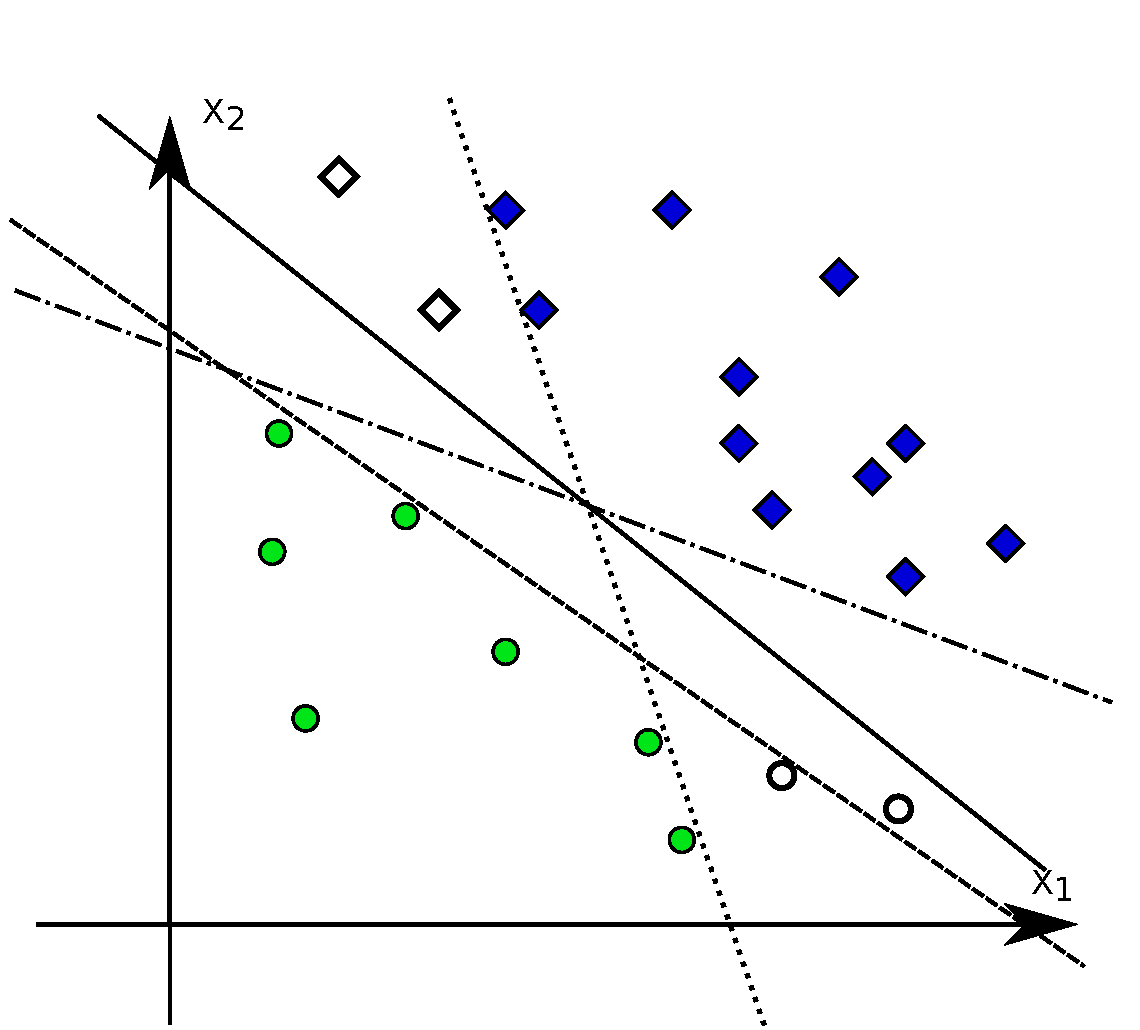
\includegraphics[scale=0.5]{figures/functions/2-different-hyperplanes}
\label{fig:hyperplanes}
\caption{Hiperpłaszczyzny separujące dwa zbiory punktów w przestrzeni dwuwymiarowej. Każda z z nich poprawnie separuje punkty ze zbioru uczącego --- zielone koła i niebieskie kwadraty. Przykłady ze zbioru testowego (puste kwadraty i kółka) są poprawnie separowane jedynie przez dwie proste (prosta narysowana linią ciągłą i prosta narysowana kropkami i kreskami).}
\end{figure}

Wynikiem uczenia klasyfikatora liniowego jest znalezienie hiperpłaszczyzny i odpowiadającej jej funkcji decyzyjnej, która przykładom ze zbioru uczącego $ (x_i, y_i) \in \Omega $ przypisuje prawidłowe etykiety, czyli dla każdego (jeśli zbiór jest liniowo separowalny), lub dla jak największej liczby przypadków $ x_i $ zachodzi  $ f_{w,b}(x_i) = y_i $. Zazwyczaj kilka hiperpłaszczyzn równie dobrze rozdziela przypadki ze zbioru uczącego, mogą się jednak one różnić zdolnością do klasyfikacji zbioru testowego, co pokazano na rysunku \ref{fig:hyperplanes}. Optymalna hiperpłaszczyzna separująca to taka, która charakteryzuje się największym marginesem, czyli odległością hiperpłaszczyzny do najbliżej położonych obserwacji \cite{scholkopf_learning_2002}.
\begin{definicjaa}
Dla hiperpłaszczyzny danej wzorem $ { x \in \Omega | \langle w, x \rangle + b = 0} $ oraz zbioru obserwacji\\
 $ {(x_1, y_1), (x_2, y_2), ..., (x_m, y_m)} $ marginesem tego zbioru od hiperpłaszczyzny nazywamy minimalną odległość hiperpłaszczyzny od punktów z tego zbioru:
	\begin{equation}
	\rho_{w,b} := \min_{i=1..m} y (\langle w, x \rangle + b) / ||w||
	\label{eq:margin}
	\end{equation}
	
\end{definicjaa}
Żeby maksymalizować margines powinniśmy minimalizować $ ||w|| $, zachowując warunek \ref{eq:canonical}. Problem znalezienia optymalnej hiperpłaszczyzny separującej zbiór przykładów  $ {(x_1, y_1), (x_2, y_2), ..., (x_m, y_m)} $ można zatem zapisać jako problem optymalizacyjny:
\begin{equation}
\begin{array}{lll}
\min\limits_{w \in \Omega, b \in \Re} &  \tau(w) = \frac{1}{2}||w||^2 & \\
\text{p.o.} &  y_i  (\langle w, x \rangle + b) \geq 1 & \text{ dla } i=1..m
\end{array}
\label{eq:primal}
\end{equation}
Ograniczenia w powyższym problemie zapewniają, że wartość funkcji decyzyjnej $ f_{w,b}(x_i) $ będzie równa $  y_i $, czyli, że hiperpłaszczyzna poprawnie odseparuje przykłady z dwóch grup. Osiągnięcie celu optymalizacji zapewnia znalezienie hiperpłaszczyzny o maksymalnym marginesie.

\begin{figure}[h]
\centering
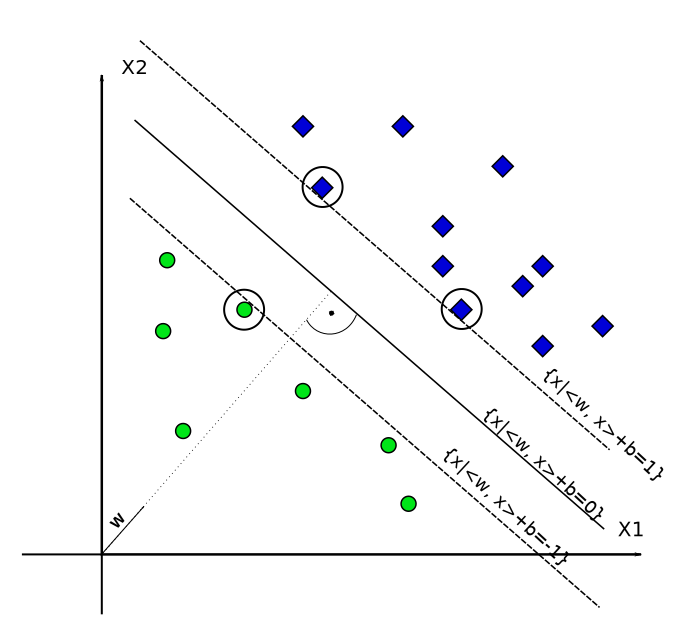
\includegraphics[scale=0.5]{figures/functions/2-margin}
\label{fig:margin}
\caption{Hiperpłaszczyzna separująca dwa zbiory punktów w przestrzeni dwuwymiarowej wraz z marginesami. Przykłady w kółku to wektory podpierające.}
\end{figure}


Powyższy problem programowania matematycznego jest podany w tak zwanej \definicja{formie prymalnej}. W praktyce rozwiązuje się wersję \definicja{dualną} problemu, która ma przyjmuje następującą postać:

\begin{definicjaa} Wersja dualna problemu znalezienia optymalnej hiperpłaszczyzny:
\begin{equation}
\begin{array}{ll}
\max\limits_{\alpha \in R^m} & W(\alpha) = \sum_{i=1}^{m} \alpha_i - \sum_{i,j=1}^{m} \alpha_i \alpha_j y_i y_j \dotp{x_i}{x_j} \\
\text{p.o.} &  \alpha_i \geq 0 , \text{ dla } i=1..m \\
& \sum_{i=1}^{m} \alpha_i y_i = 0
\end{array}
\label{eq:dual}
\end{equation}
%\begin{align}
%\max_{\alpha \in R^m} &\qquad  W(\alpha) = \sum_{i=1}^{m} \alpha_i - \sum_{i,j=1}^{m} \alpha_i \alpha_j y_i y_j \dotp{x_i}{x_j} \\
%p.o. &\qquad {}  \alpha_i \geq 0 , dla i=1..m \\
%&\qquad {} \sum_{i=1}^{m} \alpha_i y_i = 0 	
%\end{align}
\end{definicjaa}

Dla formy dualnej problemu optymalizacji funkcja decyzyjna przyjmuje postać:
\begin{equation}
f(x) = sgn \left( \sum_{i=1}^{m} y_i a_i \dotp{x}{x_i} + b \right)
\label{eq:decfn}
\end{equation}

We wzorze \ref{eq:primal} dla większości przykładów wartość współczynników $ \alpha_i $ wyniesie 0. Przykłady te nie mają wpływu na wynik optymalizacji i otrzymaną hiperpłaszczyznę. Pozostałe przykłady, dla których $ \alpha_i > 0 $ noszą nazwę \definicja{wektorów wspierających}. Leżą one dokładnie na marginesie (na hiperpłaszczyźnie wyznaczonej przez margines, czyli w przypadku kanonicznej postaci hiperpłaszczyzny separującej w odległości $ 1/||w|| $ od niej). Wektory wspierające są jedynymi przykładami ze zbioru trenującego, które należy zapamiętać w celu wyznaczenia hiperpłaszczyzny separującej. Ilość wektorów wspierających wyznacza złożoność hipotezy, którą stanowi otrzymana funkcja decyzyjna i pozwala oszacować górną granicę oczekiwanego prawdopodobieństwa błędu klasyfikacji. Górna granica prawdopodobieństwa błędu klasyfikacji klasyfikatora uczonego na zbiorze o wielkości $ m-1 $ równa się liczbie wektorów otrzymanych przy uczeniu na zbiorze o wielkości $ m $ podzielonej przez $ m $.


W przypadku, w którym dane nie są separowalne liniowo ze względu na szum, tzn. nie istnieje taka hiperpłaszczyzna, która dla danego zbioru przykładów spełnia ograniczenia ze wzoru \ref{eq:primal}, do problemu optymalizacyjnego wprowadza się tak zwane \definicja{zmienne osłabiające} (\english{slack variables}) $ \zeta_i, i=1..m $, oraz stałą $ C > 0 $, która jest parametrem algorytmu.
Wzór \ref{eq:primal} przyjmuje wówczas postać: 

\begin{equation}
\begin{array}{lll}
\min\limits_{w \in \Omega, b \in \Re} &  \tau(w) = \frac{1}{2}||w||^2 + \frac{C}{m} \sum_{i=1}^{m} \zeta_i & \\
\text{p.o.} &  y_i  (\langle w, x \rangle + b) \geq 1 - \zeta_i & \text{ dla } i=1..m \\
& \zeta_i \geq 0 & \text{ dla } i=1..m \\
\end{array}
\label{eq:primal-c}
\end{equation}

Natomiast wzór \ref{eq:dual}:
\begin{equation}
\begin{array}{ll}
\max\limits_{\alpha \in R^m} & W(\alpha) = \sum_{i=1}^{m} \alpha_i - \sum_{i,j=1}^{m} \alpha_i \alpha_j y_i y_j \dotp{x_i}{x_j} \\
\text{p.o.} & 0 \leq \alpha_i \leq \frac{C}{m} , \text{ dla } i=1..m \\
& \sum_{i=1}^{m} \alpha_i y_i = 0
\end{array}
\label{eq:dual-c}
\end{equation}

\subsection{Maszyny wektorów wspierających}


\begin{figure}[h]
\centering
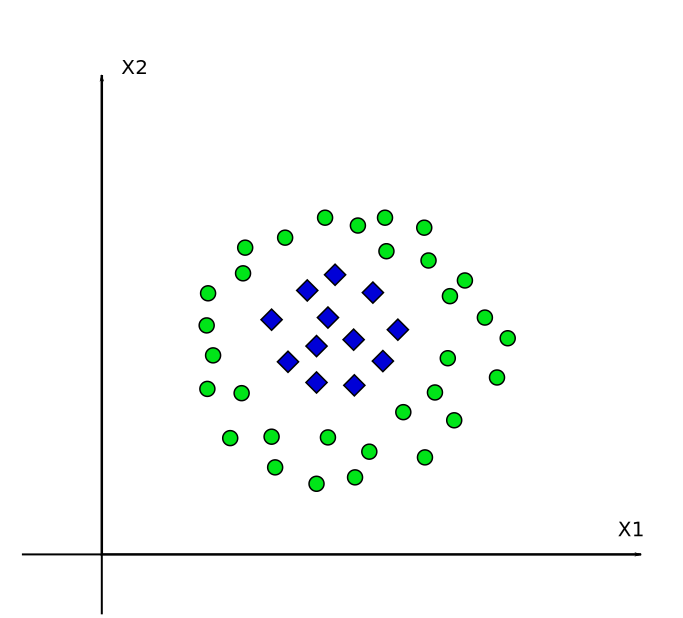
\includegraphics[scale=1]{figures/functions/2-nonlinear}
\label{fig:nonlinear}
\caption{Zbiór danych opisanych w przestrzeni 2D. Klas (niebieskie kółka - klasa $+1$, zielone krzyżyki - klasa $-1$) nie da się odseparować za pomocą hiperpłaszczyzny}
\end{figure}

\begin{figure}[h]
\centering
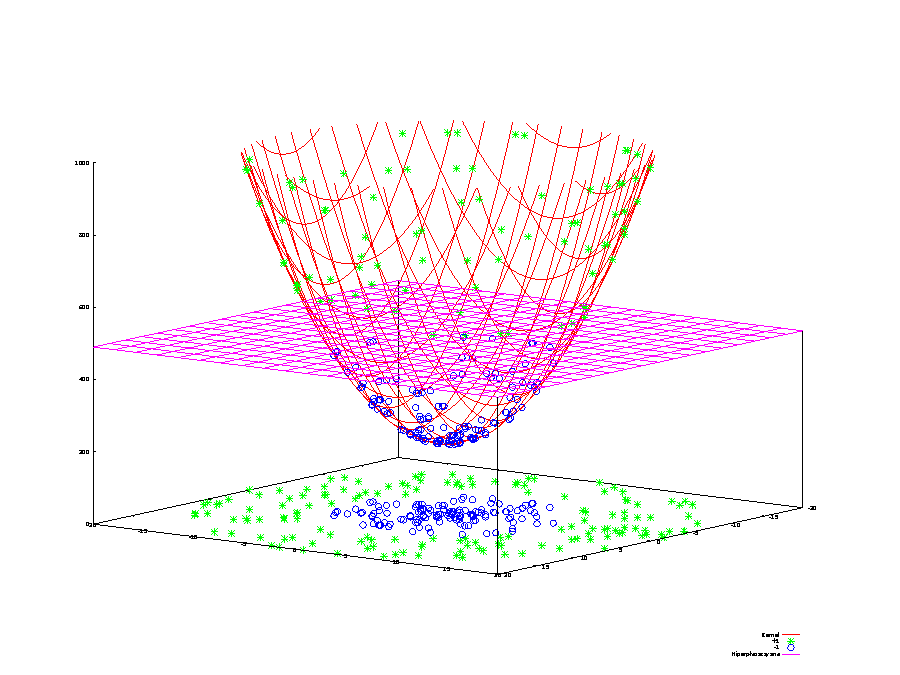
\includegraphics[scale=0.8]{figures/functions/2-transform}
\label{fig:transform}
\caption{Zbiór z rysunku \ref{fig:nonlinear} po dokonaniu transformacji do przestrzeni 3-wymiarowej. Na wysokości 0 pokazano dane przed transformacją. W nowej przestrzeni klasy mogą być rozdzielone hiperpłaszczyzną.}
\end{figure}

\begin{figure}[h]
\centering
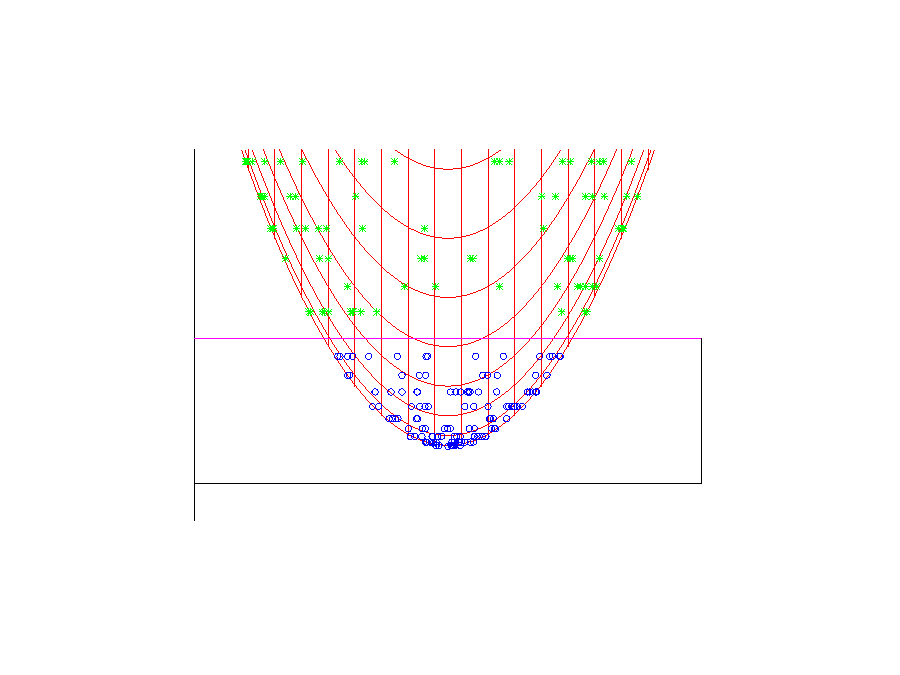
\includegraphics[scale=0.8]{figures/functions/2-transform-side}
\label{fig:transform-side}
\caption{Zbiór z rysunku \ref{fig:nonlinear} po dokonaniu transformacji do przestrzeni 3-wymiarowej, rzut wzdłuż osi X}
\end{figure}


Opisane powyżej klasyfikatory są w stanie klasyfikować tylko dane, które są separowalne liniowo. Jeśli dane cechuje pewna inna niż liniowa zależność między wartościami atrybutów decyzyjnych i warunkowych (na przykład taka jak przedstawiona na rysunku \ref{fig:nonlinear}), to klasyfikator liniowy nie poradzi sobie z ich klasyfikacją.
Aby rozwiązać ten problem można dokonać mapowania danych wejściowych do przestrzeni o większej liczbie wymiarów, w której te dane mogą stać się liniowo separowalne. Na rysunku \ref{fig:transform} pokazano dane z rysunku \ref{fig:nonlinear} po transformacji do przestrzeni trójwymiarowej za pomocą funkcji wielomianowej. Jak widać w nowej przestrzeni dane są separowalne przez hiperpłaszczyznę, co widać dokładnie na rysunku \ref{fig:transform-side}.

Mapowanie z oryginalnej przestrzeni atrybutów do nowej przestrzeni jest dokonywane przez funkcję $ \Phi: \Omega^m \mapsto \Omega^{m+k} $, która dane n-wymiarowe zamienia w dane n+k-wymiarowe. Na przykład mapowanie wektora $x = \left[ x_1, x_2 \right] $ z przestrzeni 2-wymiarowej do przestrzeni 3-wymiarowej może wyglądać następująco:
% $ \Phi(x) = \Phi(\left[x_1]_1, [x_1]_2 \right]) = \left[ {[x_1]_1}^2, {[x_1]_2}^2, [x_1]_1 [x_1]_2 \right] $
 $ \Phi(x) = \Phi(\left[x_1, x_2 \right]) = \left[ x_1^2, x_2^2, x_1 x_2 \right] $. Aby zastosować mapowanie w klasyfikatorze wystarczy zamienić wszystkie wystąpienia wektorów wynikiem ich mapowań, czyli na przykład cel optymalizacji ze wzoru \ref{eq:dual} przyjąłby postać:

\begin{equation}
\max\limits_{\alpha \in R^m}  W(\alpha) = \sum_{i=1}^{m} \alpha_i - \sum_{i,j=1}^{m} \alpha_i \alpha_j y_i y_j \dotp{\Phi(x_i)}{\Phi(x_j)}
\label{eq:dual-k-target}
\end{equation}

natomiast funkcja decyzyjna ze wzoru \ref{eq:decfn}:
\begin{equation}
f(x) = sgn \left( \sum_{i=1}^{m} y_i a_i \dotp{\Phi(x)}{\Phi(x_i)} + b \right)
\end{equation}

\FloatBarrier

Powyższe podejście charakteryzuje się dużą złożonością obliczeniową. Zarówno obliczanie mapowania dla każdego przykładów jak i obliczenie iloczynu skalarnego przykładów w nowej przestrzeni, która może mieć bardzo dużo wymiarów, stanowi spory narzut obliczeniowy. Dokonywanie wszystkich mapowań a następnie obliczanie ich iloczynu nie jest jednak konieczne, można obie te operacje wykonać w jednym kroku, stosując tak zwany \english{Kernel Trick} \cite{Boser:1992:TAO:130385.130401}. Polega on na zastosowaniu podstawienia $ \dotp{\Phi(x)}{\Phi(x')} \mapsto k(x, x') $ gdzie $ k(x,x') $ to \definicja{funkcja jądrowa} (\english{kernel}). Po zastosowaniu \emph{kernel trick} otrzymujemy następujący problem optymalizacyjny:

\begin{equation}
\begin{array}{ll}
\max\limits_{\alpha \in R^m} & W(\alpha) = \sum_{i=1}^{m} \alpha_i - \sum_{i,j=1}^{m} \alpha_i \alpha_j y_i y_j k(x_i, x_j) \\
\text{p.o.} &  \alpha_i \geq 0 , \text{ dla } i=1..m \\
& \sum_{i=1}^{m} \alpha_i y_i = 0
\end{array}
\label{eq:dual-k}
\end{equation}

oraz następującą funkcję decyzyjną: 

\begin{equation}
f(x) = sgn \left( \sum_{i=1}^{m} y_i a_i k(x, x_i) + b \right)
\label{eq:decfn-k}
\end{equation}

\subsection{Funkcje jądrowe}

Funkcję jądrowe pozwalają obliczyć iloczyn skalarny wyników mapowania ($ \Phi() $) dwóch wektorów ($ x, x' $) do wysoko wymiarowej przestrzeni atrybutów ($ \Omega^{m+k} $), bez bezpośredniego dokonywania mapowania:
$$ \Phi: \Omega^m \mapsto \Omega^{m+k} $$
$$ \dotp{\Phi(x)}{\Phi(x')} \mapsto k(x, x')  $$

Najczęściej używane funkcje jądrowe to:	
\begin{itemize}
	\item Wielomianowa: $ k(x, x') = \langle x,y \rangle ^d $
	\item Gausowska (RBF): $k(x, x') =  e^{-\sigma*||x-y||^2} $	
	\item Sigmoidalna: $ k(x, x') = \tanh(\gamma \langle x,y \rangle + \tau) $
\end{itemize}

Jako funkcję jądrowe w SVM można użyć jednak dowolnej symetrycznej funkcji, która jest dodatnio określona (\english{positive definite}), czyli dla której macierz:
$$ K_{ij} := k(x_i, x_j) $$
spełnia warunek:
\begin{equation}
\label{eq:pd}
\sum_{i,j}c_i c_j K_{ij} \geq 0
\end{equation} 
dla wszystkich $ c_i \in \Re $
co jest równoważne temu, że jej wszystkie wartości własne są dodatnie \cite{scholkopf_learning_2002}.

Spełnienie powyższego warunku gwarantuje, że rozwiązywany problem programowania matematycznego będzie wypukły, czyli będzie miał tylko jedno minimum lokalne, będące zarazem minimum globalnym.
Dla funkcje jądrowych, które nie są dodatnio określone, rozwiązywany w SVM problem wciąż może być wypukły, pod warunkiem, że są one warunkowo dodatnio określone (\english{conditionally positive definite}). Jest to możliwe dzięki ograniczeniu \ref{eq:dual-k}, które wyklucza pewne wartości współczynników $ \alpha $. Wyniki eksperymentalne pokazują, że w praktyce funkcje, które są jedynie warunkowo dodatni określone, mogą dawać równie dobre wyniki co funkcje dodatnio określone \cite{2005Boughorbel}. Funkcja jest warunkowo dodatnio określona, jeśli spełnia warunek ze wzoru \ref{eq:pd} przy czym $ \sum_{i,j} c_i = 0 $.


Funkcje jądrowe cechuje własność domknięcia ze względu na pewne operacje. Oznacza to, że funkcje powstałe poprzez połączenie poprawnych funkcji jądrowych za pomocą tych operatorów również są poprawnymi funkcjami jądrowymi \cite{Shawe-Taylor:2004:KMP:975545}. Jeżeli $ k_1(x, z) $ i $ k_2 (x,z) $ są kernelami, to również poniższe funkcje są kernelami:

\begin{equation}
\begin{array}{ll}
	k(x, x') = k_1(x,z) + k_2(x,x') \\
	k(x, x') = k_1(x,z) \times k_2(x,x') \\
	k(x, x') = a \times k_1(x,x')) \\
	k(x, x') = e^{k_2(x,x')} \\
%	k(x, x') = e^{- \frac{|| x - x' ||^2}{2\sigma^2	} }
	k(x, x') = p(k_1(x,x')) 	
\end{array}
\label{eq:kernelclosure}
\end{equation}

gdzie $ a \in \mathbb{R}^{+} $, a $ p() $ to wielomian o dodatnich współczynnikach.


\subsubsection{Algorytmy wykorzystujące funkcje jądrowe}
\emph{SVM} nie jest jedynym algorytmem wykorzystującym funkcję jądrowe do dokonania mapowania danych do wysoko wymiarowych przestrzeni. Ich użycie jest zasadne wszędzie tam, gdzie zamiast działać wprost na wejściowych wektorach danych można operować na ich iloczynach skalarnych \cite{scholkopf_learning_2002}. W związku z tym funkcje jądrowe znalazły zastosowania w wielu algorytmach, zwanych zbiorczo jak metody jądrowe (\english{kernel methods}):
\begin{itemize}
	\item \emph{Kernel-NN} \cite{Yu:2002:KNA:607789.607852} --- modyfikacja \definicja{k-NN} korzystająca z funkcji jądrowych do obliczania odległości między przykładami
	\item definicja{k-PCA} \cite{scholkopf_learning_2002} --- modyfikacji algorytmu analizy głównych składowych \definicja{Principal Component Analysis }(\akronim{PCA}), który może służyć m.in. do konstrukcji cech opisujących przykłady, klasyfikowane potem za pomocą jakiegoś algorytmu klasyfikacji.
	\item \definicja{Support Vector Regression} (\definicja{SVR}) --- regresja za pomocą SVM
	\item \definicja{Kernel Fisher Discriminant} (\akronim{KFD}) \cite{scholkopf_learning_2002} --- zastosowanie funkcji jądrowych w liniowym dyskryminatorze Fishera, który może służyć do redukcji wymiarów opisujących przykłady i/lub do klasyfikacji.
\end{itemize}

\subsection{Klasyfikacja więcej niż dwóch klas}
Klasyfikator SVM jest ze swej natury klasyfikatorem binarnym, to znaczy potrafi separować jedynie dwie klasy przykładów. W praktyce jednak wiele problemów klasyfikacji dotyczy zbiorów, w których wyróżniono więcej niż dwie klasy. Aby zastosować SVM do rozwiązania takich problemów stosuje się zazwyczaj jedną z dwóch technik: \definicja{jeden przeciw wszystkim} (\english{One versus the Rest}) oraz \definicja{klasyfikacja parami} (\english{pairwise classification}). 

\subsubsection{Jeden przeciw wszystkim}
Metoda \definicja{jeden przeciw wszystkim} polega na nauczeniu $ M $ klasyfikatorów binarnych, gdzie $ M $ oznacz liczbę klas. Każdy z nich separuje jedną klasę od pozostałych $ M-1 $ klas, traktując te ostatnie jak jedną klasę. Klasyfikacja polega na zastosowaniu wszystkich $ M $ klasyfikatorów na testowanym przykładzie i wybraniu tego, który maksymalizuje wartość ze wzoru \ref{eq:decfn-k}, przed zastosowaniem funkcji $ sgn $, czyli:

$$
\begin{array}{ll}
 & argmax_{j=1..M} g^j(x) \\
\text{gdzie } & g^j(x) = \sum_{1=1}^m y_ia_i^j k(x, x_i) + b^j
\end{array}
$$



Jako wady tej metody wymienia się to, że pod-problemy przez nią rozwiązywane są niesymetryczne (jeśli w wyjściowym problemie dystrybucja przykładów do klas jest równomierna, to w każdym podproblemie klasa agregująca "pozostałe" klasy jest $ M-1 $ razy większa ). Z problemem asymetryczności lepiej radzi sobie druga z wymienionych metod.

\subsubsection{Klasyfikacja parami}
Metoda \definicja{klasyfikacji parami} polega na stworzeniu wszystkich możliwych kombinacji klasyfikatorów binarnych: dla każdej z $ M $ klas tworzy się $ M-1 $ klasyfikatorów oddzielających ją od poszczególnych klas, co daje łącznie $ (M-1)*M/2 $ klasyfikatorów. Każdy z nich uczony jest tylko na przykładach należących do 2 wybranych klas. Klasyfikacja przykładu odbywa się poprzez głosowanie: każdy z $ (M-1)*M/2 $ klasyfikatorów oddaje głos na klasę, do której przypisał dany przykład. Przykładowi przypisuje się klasę, która zdobyła największą liczbę głosów.
Choć w tej metodzie liczba klasyfikatorów, które trzeba nauczyć a potem użyć do klasyfikacji jest znacznie większa niż w metodzie \definicja{jeden przeciw wszystkim}, to jednak uczenie odbywa się na mniejszej liczbie przykładów a klasyfikacja z użyciem mniejszej liczby wektorów wspierających, co może przyspieszyć sprawia, że etapy te przebiegają szybciej niż w metodzie \definicja{jeden przeciw wszystkim}. Ponieważ jednak liczba klasyfikatorów rośnie potęgowo względem liczby klas $ M $, to dla dużych $ M $ \definicja{klasyfikacja parami} może okazać się wolniejsza niż \definicja{jeden przeciw wszystkim}.


\section{Obliczenia ewolucyjne}

\definicja{Obliczenia ewolucyjne} (\english{Evolutionary computation} (\akronim{EC})) to grupa inspirowanych biologicznie technik obliczeniowych. 
Algorytmy należące do tej grupy to \definicja{Algorytmy Ewolucyjne} (\english{Evolutionary Algorithms} (\akronim{EA})). Algorytmy te stanowią rodzaj metaheurystyk, czyli uniwersalnych algorytmów służących rozwiązywaniu różnych problemów optymalizacji, często wykorzystujących w trakcie działania bardziej specyficzne algorytmy. Algorytmy ewolucyjne wyróżnia wśród innych metaheurystyk między innymi przynależność do grupy algorytmów populacyjnych, które charakteryzują się równoległym przeszukiwaniem wielu rozwiązań, między którymi zachodzą interakcje wpływające na ocenę poszczególnych rozwiązań jak i kierunek ich zmian. Idea obliczeń ewolucyjnych czerpie swoje inspiracje z biologicznych teoriach ewolucji, z nich również zapożycza terminologię. Poniżej przedstawiono znaczenie terminów używanych w kontekście obliczeń ewolucyjnych \cite{Luke2009Metaheuristics}:

\begin{itemize}
	\item \definicja{osobnik} (\english{individual}) --- jedno z potencjalnych rozwiązań problemu
	\item \definicja{genotyp} (\english{genotype}) --- dane opisujące osobnika, podlegające procesom mutacji i krzyżowania
	\item \definicja{relacja rodzic-potomek} (\english{parent-parent}) --- potomek to osobnik powstały poprzez mutację rodzica lub w wyniku krzyżowania dwóch rodziców
	\item \definicja{mutacja} (\english{mutation}) --- zmiana genotypu pojedynczego osobnika w wyniku której powstaje osobnik o nowym genotypie
	\item \definicja{krzyżowanie} (\english{crossover}) --- stworzenie jednego lub więcej nowych osobników, których genom jest kombinacją genomów rodziców
	\item \definicja{populacja} (\english{population}) --- zbiór osobników
	item \definicja{pokolenie} (\english{generation}) --- kompletny cykl operacji wykonanych na pokoleniu, również pokolenie będące jego wynikiem
	\item \definicja{przystosowanie / wartość funkcji przystosowania} (\english{fitness}) --- wartość określająca jakość osobnika ze względu na cel optymalizacji przyjęty w rozwiązywanym problemie
	\item \definicja{selekcja} (\english{selection}) --- wybór podzbioru osobników z populacji na podstawie ich przystosowania
	\item \definicja{powielanie} --- utworzenie nowego osobnika poprzez skopiowanie istniejącego osobnika bez zmian
	\item \definicja{reprodukcja} (\english{breeding}) --- proces tworzenia nowego pokolenia (nowej generacji) osobników z osobników już istniejących poprzez procesy mutacji, krzyżowania i selekcji.
\end{itemize}

\begin{figure}[h]
\centering
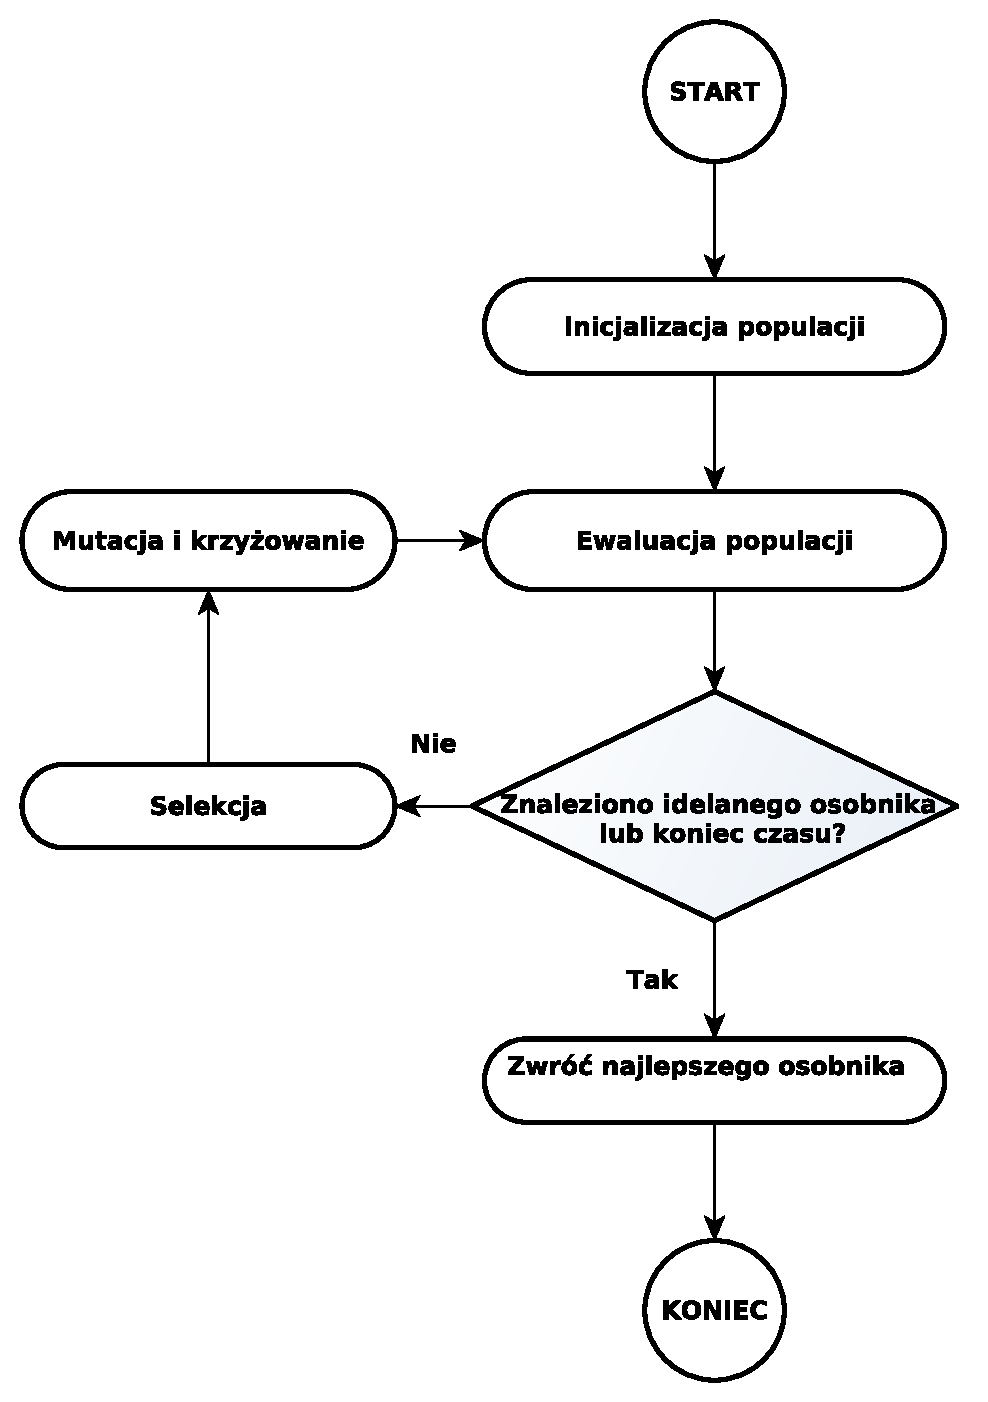
\includegraphics[scale=0.5]{figures/graphs/ea}
\caption{Diagram przepływu algorytmu ewolucyjnego GP.\label{fig:ea}}
\end{figure}

Przebieg typowego algorytmu ewolucyjnego przedstawiono na rysunku \ref{fig:ea}, poniżej przedstawiono jego opis:
\begin{quote}
	\begin{enumerate}
	\item Utwórz początkową populację osobników korzystając z losowego mechanizmu lub użyj istniejącej populacji
	\item \label{ewaluacja} Oblicz wartość \textit{funkcji dopasowania} każdego osobnika z populacji (dokonaj ewaluacji populacji).
	\item Jeśli znaleziono idealnego osobnika (wartość fitness wyniosła 1 ) lub skończył się czas, zwróć najlepszego znalezionego dotąd osobnika
	\item Dokonaj selekcji osobników
	\item Utwórz nową populację poprzez mutację, krzyżowanie lub powielanie wybranych w poprzednim kroku osobników
	\item Wróć do punktu \ref{ewaluacja}
	\end{enumerate}
\end{quote}



\subsubsection{Selekcja}
Selekcja polega na wybraniu podzbioru $ P $ osobników z populacji. Jej celem jest promowanie dobrych rozwiązań, które powstały w wyniku generowania nowych osobników, mutacji oraz krzyżowania. Dzięki dokonywaniu selekcji geny osobników lepiej przystosowanych do rozwiązania postawionego przed algorytmem problemu są "przekazywane dalej", biorąc udział w tworzeniu nowych osobników. "Dobroć" rozwiązań jest oceniana poprzez funkcję przystosowania, która przyjmuje wartości z przedziału $ \langle 0, 1 \rangle $, gdzie 0 oznacza najgorsze rozwiązanie a 1 rozwiązanie idealne.
Najprostszym, "naiwnym", sposobem przeprowadzenia selekcji jest wybór z niej określonej liczby osobników o najwyższej wartości fitness. Rozwiązanie to jednak nie jest optymalne --- czasami pożądane fragmenty genotypu są "ukryte" w osobnikach, które nie osiągają najwyższych wartości fitness, dlatego warto dopuścić również niektóre ze "słabszych" osobników do etapu krzyżowania.
Głównym parametrem wpływającym na proces selekcji jest \definicja{napór selekcyjny}. Im większy napór selekcyjny tym trudniej osobnikom przejść selekcję co prowadzi do ujednolicania się osobników w populacji, ponieważ do następnego pokolenia przechodzi tylko wąska grupa najlepszych osobników, zmniejszając tym samym pulę genów pokolenia. Zmniejszanie się różnorodności jest niepożądanym procesem, ponieważ prowadzi do stagnacji procesu ewolucyjnego --- kiedy wszystkie osobniki mają ten sam genotyp jedyne zmiany w populacji możliwe są poprzez mutację. Stagnacja procesu ewolucyjnego oznacza, że populacja z pokolenia na pokolenie się nie zmienia, ponieważ przez etap selekcji przechodzą zawsze te same, podobne do siebie osobniki. Jest to równoważne z utknięciem w optimum lokalnym (które może, choć nie musi być optimum globalnym rozwiązywanego problemu). Dlatego, żeby nie dopuścić do zbyt szybkiego ujednolicenia populacji stosuje się różne, bardziej wyrafinowanej niż opisany powyżej "naiwny", algorytmy selekcji:

%Tutaj opisy selekcji ze strony 57 ECJ, 41 Essentials 

\begin{itemize}

\item \definicja{ruletka} --- metoda ruletki, zwana też wyborem losowym powtórzeniami \english{Fitness-Proportionate Selection} polega na losowaniu osobników z prawdopodobieństwem wylosowania proporcjonalnym do ich wartości fitness. Metaforycznie można ją przedstawić w ten sposób, że każdemu osobnikowi przypisuje się pole na kole od ruletki o wielkości proporcjonalnej do jego wartości fitness i kręcąc ruletką losuje ustaloną liczbę osobników. 
Ta metoda selekcji dopuszcza wybranie jednego osobnika kilka razy a także umożliwia przypuszczenie osobników o małych wartościach fitness, co jest korzystne dla różnorodności populacji. Wadą tej metody jest ukryte w niej założenie o ilorazowym charakterze skali wartości fitness --- osobnik A o k-krotnie większym fitness od osobnika B będzie średnio wybierany k razy częściej niż osobnik B, choć w ogólności nie musi być tak, że k-krotnie większy fitness oznacza k-krotnie lepszego lub pożądanego z punktu widzenia puli genów populacji osobnika. Z tym problemem radzi sobie następna opisana metoda.

\item \definicja{turniej} --- metoda turniejowa (\english{tournament selection}) jest najbardziej popularną i jednocześnie najprostszą z metod selekcji \cite{Luke2009Metaheuristics}. Polega na losowaniu ze zwracaniem $ t $ osobników i wybraniu tego, który ma największą wartość fitness. Parametr $ t $ to tak zwany \definicja{rozmiar turnieju}, zwiększając go zwiększamy presję selekcyjną. Dla $ t = 1 $ selekcja sprowadza się do losowego wyboru osobników, dla $ t = P $ otrzymamy populację składającą się z $ P $ kopii osobnika o najwyższym fitness.	

\end{itemize}


\subsubsection{Krzyżowanie}
Osobniki wybrane w procesie selekcji z ustalonym jako parametr procesu ewolucyjnego prawdopodobieństwem ulegają krzyżowaniu, czyli wymieszaniu ich genotypów, w czego wyniku powstaje nowy osobnik o przypuszczalnie nieobecnym wcześniej genotypie.

\subsubsection{Mutacja}
Mutacja polega na losowej, zazwyczaj nieznacznej, zmianie genotypu osobnika. Wpływa korzystnie na różnorodność populacji wprowadzając fragmenty genomu, które mogły wcześniej nie być obecne w puli genów populacji. Mutacja podobnie jak krzyżowanie jest stosowana z pewnym prawdopodobieństwem. Im to prawdopodobieństwo większe a zmiany dokonywane przez mutację bardziej rozległe, tym bardziej "eksploratywny" staje się algorytm ewolucyjny --- trudniej mu "utknąć" w lokalnym optimum.

\subsubsection{Genotyp}
Poszczególne algorytmy ewolucyjne różnią się od siebie przede wszystkim ze względu na sposób reprezentacji osobników i powiązane z nim metody mutacji i krzyżowania. Selekcja osobników także może przebiegać na różne sposoby. Opisanie wszystkich możliwych parametrów i metod używanych w algorytmach ewolucyjnych nie jest celem tej pracy, ich opis można znaleźć na przykład w \cite{Luke2009Metaheuristics}. Poniżej opisano jeden z rodzajów algorytmów ewolucyjnych jaką jest programowanie genetyczne, ze względu na jej wykorzystanie w niniejszej pracy.


%%%%%%%%%%%%%%%%%%%%%%%%%%%%%%%%%%%%%%%%%%%%
\subsection{Programowanie genetyczne}

\definicja{Programowanie genetyczne} (\akronim{GP}, \english{Genetic Programming}) to rodzaj algorytmów ewolucyjnych, które wyróżniają się specyficzną reprezentacją --- ewolucji podlegają wyrażenia reprezentowane za pomocą drzew, na przykład wyrażenia matematyczne, logiczne lub kod programu komputerowego. Najczęściej w definicji programowania genetycznego podaje się właśnie ten ostatni rodzaj osobników \cite{Luke2009Metaheuristics} \cite{Poli:2008:FGG:1796422}, lecz ewolucja innych wyrażeń reprezentowanym za pomocą drzew przebiega w algorytmie programowania genetycznego w identyczny sposób.

\begin{figure}[h]
\centering
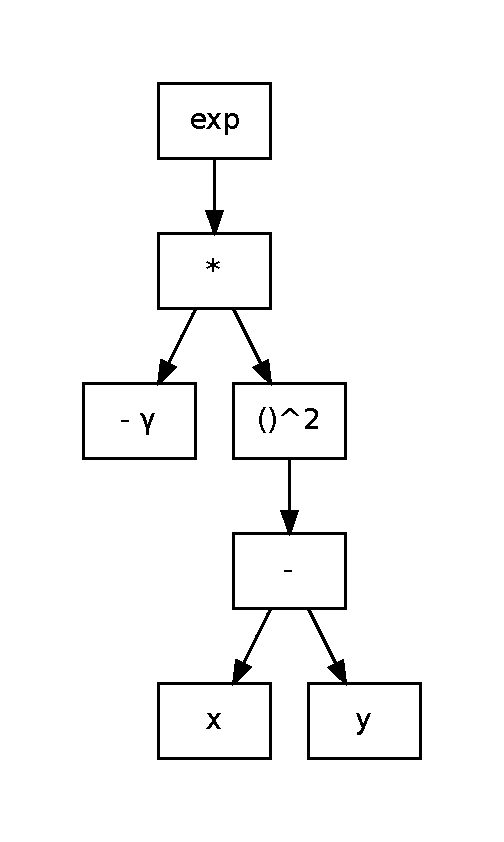
\includegraphics[scale=0.6]{figures/graphs/2-tree}
\caption{Przykładowe drzewo, które może być wynikiem działania algorytmu GP. Drzewo przestawia wyrażenie $ e^{-\gamma*(x-y)^2} $ \label{fig:2-tree}}
\end{figure}

Drzewo generowane przez algorytm GP (np. takie jak pokazane na rysunku \ref{fig:2-tree})  składa się z \emph{terminali} (liście) oraz \emph{funkcji} (węzły wewnętrzne oraz korzeń). Terminale to wartości wejściowe generowanego wyrażenia --- stałe i zmienne --- na rysunku są to zmienne $ x $ i $ y $ oraz stała $ \lambda $. Funkcje to operacje wykonywane wartościach pochodzących z terminali lub innych funkcji, w przypadku drzewa z rysunku \ref{fig:2-tree} są to: funkcja wykładnicza $ exp() $ oraz funkcja potęgowa (korzeń). Każdy węzeł wewnętrzny posiada łuk(i) wejściowe, którymi funkcja "pobiera" wartości swoich argumentów oraz łuk wyjściowy, którym przekazuje wartość do kolejnych funkcji (lub w przypadku korzenia zwraca wartość obliczoną przez całe wyrażenie).

\subsubsection{Inicjalizacja populacji}
\label{ssec:inicjalizacja}
Wybranie sposobu inicjalizacji populacji sprowadza się do określenia metody losowego generowania osobników. Drzewa są budowane przez łączenie ze sobą funkcji wybieranych ze \definicja{zbioru funkcji} oraz terminali. Każda funkcja ma określoną liczbę argumentów oraz opcjonalnie typ danych wejściowych i wyjściowych. W najprostszym przypadku wszystkie węzły drzewa operują na tych samych typach danych, wtedy nie narzuca się ograniczeń na to które węzły mogą się ze sobą łączyć. Jeśli jednak zbiór funkcji i terminali jest heterogeniczny ze względu na wartości typów danych, konieczne jest wprowadzenie ograniczeń. Odmiana \definicja{GP}, w której każda funkcja ma zdefiniowane typy danych, na których operuje nazywany jest \definicja{Strongly Typed GP \akronim{STGP}}.
Kolejnym ograniczeniem najczęściej narzucanym na generowane drzewa jest ich głębokość, czyli odległość od najdalszego liścia do korzenia. Ze względu na to ograniczenie wyróżnia się 3 podstawowe metody generowania osobników:
\begin{itemize}
	\item \definicja{full} --- generuje drzewa o maksymalnej dozwolonej głębokości, w których każdy liść jest oddalony od drzewa o maksymalną odległość. Genrowanie polega na budowaniu drzewa zaczynając od korzenia poprzez losowanie kolejnych funkcji ze zbioru funkcji i dołączenie ich do funkcji już istniejących w drzewie, tak długo aż wszystkie gałęzie osiągną oczekiwaną głębokość. Na końcu dla każdej gałęzi losuje się kończący ją terminal.
	\item \definicja{grow} --- w tej metodzie węzły budujące drzewo są losowane z obu zbiorów: funkcji i terminali. Dzięki temu, w przypadku wylosowania terminala dana gałąż kończy swój wzrost i otrzymujemy z gałęziami o potencjalnie zróżnicowanej długości.
	\item \definicja{ramped half-and-half} --- w metodzie tej połowę populacji inicjalizacje się za pomocą metody \definicja{grow} a druga połowę za pomocą algorytmu \definicja{full}, dodatkowo zmieniając maksymalną możliwą głębokość. Metoda ta pozwala otrzymać populację najbardziej urozmaiconą pod względem kształtu i wielkości drzew.
\end{itemize}


\subsubsection{Krzyżowanie}
Najpowszechniejsza metoda krzyżowania w programowaniu genetycznym to \definicja{krzyżowanie poddrzew \english{subtree crossover}}. Polega ona na zamianie poddrzew dwóch rodziców w czego wyniku powstaje dwóch potomków. Poddrzewa otrzymuje się poprzez wybór punktu cięcia, w którym poddrzewo jest odcinane od rodzica. Przykładowy proces krzyżowania zilustrowano na rysunku \ref{fig:2-cross}.

\begin{figure}[h]
\centering
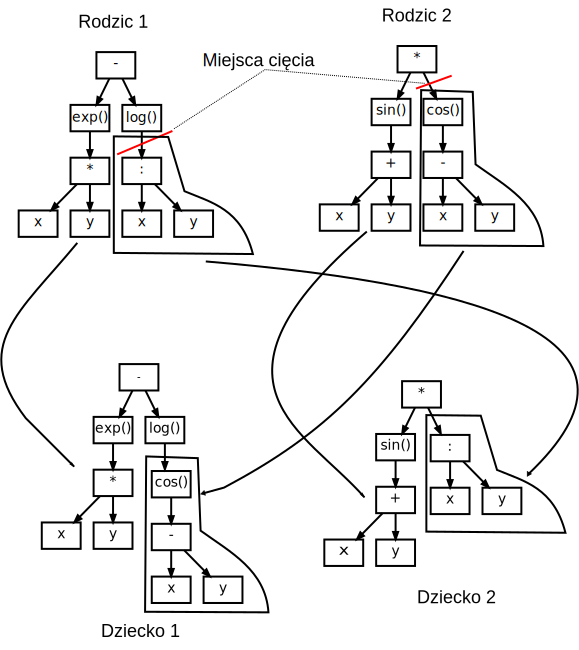
\includegraphics[scale=0.8]{figures/graphs/2-cross-both}
\label{fig:2-cross}
\caption{Krzyżowanie drzew. U góry pokazano drzewa rodziców, punkty cięcia zaznaczono czerwonymi kreskami. Na dole widać dwóch potomków będących wynikiem krzyżowania.}
\end{figure}

\subsubsection{Mutacja}
Mutacja drzewa polega na zamianie jego losowo wybranego fragmentu (poddrzewa) przez losowo wygenerowane drzewo odpowiedniej długości. Pod tym względem mutacja przypomina krzyżowanie, z tą różnicą, że odcięty fragment mutowanego drzewa jest zastępowany przez losowo wygenerowane drzewo a nie poddrzewo pochodzące od drugiego rodzica. Przykładową mutację drzewa pokazano na rysunku \ref{fig:2-mutation}.

\begin{figure}[h]
\centering
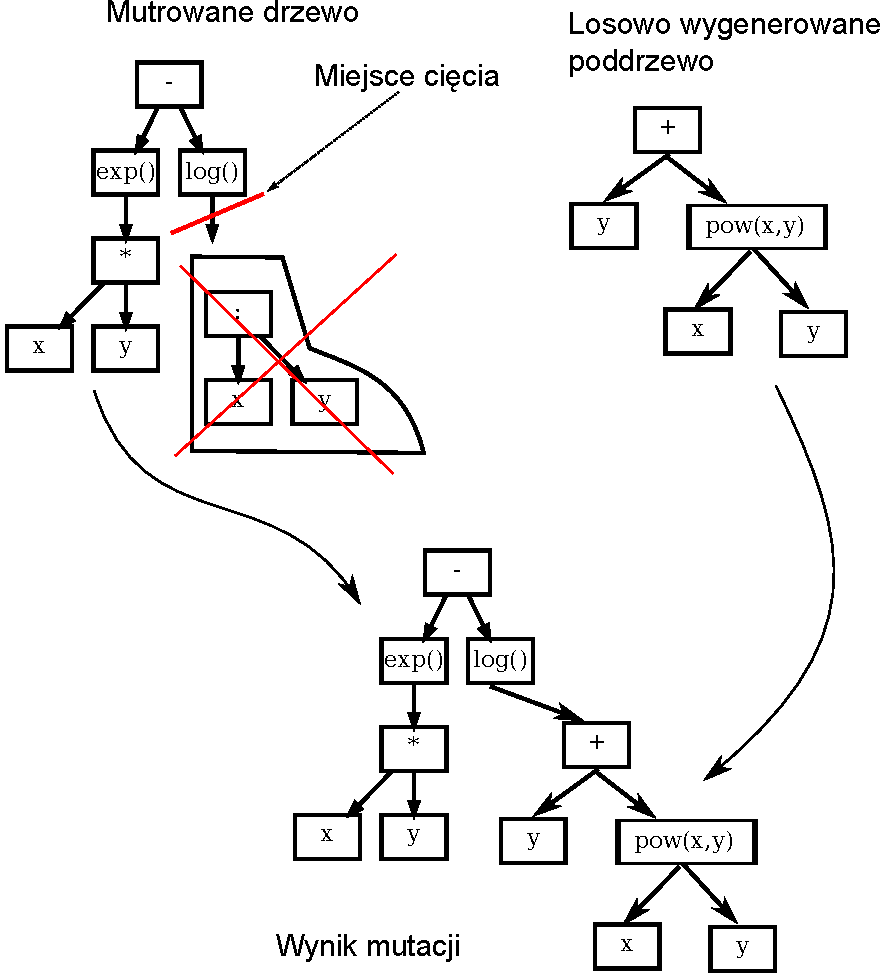
\includegraphics[scale=0.8]{figures/graphs/2-mutation}
\label{fig:2-mutation}
\caption{Przykładowa mutacja drzewa. U góry po lewej pokazano drzewo poddawane mutacji, u góry po prawej losowo wygenerowane poddrzewo, na dole wyniki mutacji. Odcinana część mutowanego drzewa (na rysunku przekreślona) zostaje odrzucona (nie jest już nigdzie wykorzystywana).} 
\end{figure}

\subsubsection{Selekcja}
Selekcja w GP może być dokonywana jedną z metod używanych w innych algorytmach ewolucyjnych, jednak istnieją też metody specyficzne dla algorytmów GP. Jednym z problemów programowania genetycznego jest zjawisko \definicja{przerostu} (\english{bloat}). Polega ono na tym, że drzewa powstałe w wyniku procesu ewolucyjnego mogą być bardzo duże, co nie jest pożądaną cechą --- większe drzewo dłużej oblicza zwracaną wartość, zajmuje więcej miejsc w pamięci. Dlatego wielkość drzew należy ograniczać, jeśli wzrost drzewa nie prowadzi do zwiększenia wartości funkcji dopasowania.
Wielkość generowanych drzew może być regulowana przez kilka mechanizmów. Najprostszy z nich to proste ograniczenie na maksymalną głębokość drzewa --- podczas inicjalizacji lub mutacji wzrost drzewa(poddrzewa) jest zatrzymywany kiedy osiągnie ono maksymalną głębokość. Algorytm może również odrzucać zbyt duże drzewa powstałe podczas krzyżowania.
Grupa bardziej wyrafinowanych mechanizmów o angielskiej nazwie \textit{parsimony pressure}, promuje mniejsze drzewa podczas selekcji. Do grupy tej należą algorytmy \cite{sean_ecj_2010}:
\begin{itemize}
	\item \definicja{Selekcja turniejowa leksykograficzna} --- przebiega tak samo jak selekcja turniejowa, ale w przypadku, gdy porównywane są dwa osobniki o równej wartości fitness, wygrywa ten, który jest mniejszy
	\item \definicja{Selekcja turniejowa leksykograficzna z koszykami} (\english{bucket lexicographic tournament selection}) --- osobniki w populacji sortowane są według przystosowania, następnie grupuje się je w N "koszyki". Następnie selekcja przebiega według zasad selekcji turniejowej, z tym, że porównuje się nie przystosowanie osobników, ale koszyk, do którego są przypisane. W przypadku gdy w turnieju porównywane są dwa osobniki z tego samego koszyka wygrywa ten, który jest mniejszy.
	\item \definicja{Selekcja turniejowa proporcjonalna} (\english{proportional tournament selection}) --- przebiega tak samo jak selekcja turniejowa, z tym, że z pewnym prawdopodobieństwem osobniki są porównywane według przystosowania albo według wielkości
	\item \definicja{Podwójna selekcja turniejowa} (\english{double tournament selection}) --- selekcja odbywa się w dwóch rundach --- najpierw w N turniejach wybiera się N osobników, według ich wielkości (przystosowania), następnie tych N osobników bierze udział w turnieju, w którym porównywani są według przystosowania (wielkości)
	\item \definicja{\english{Tarpeian statistics}} --- nie jest to metoda selekcji, lecz sposób przypisania wartości przystosowania. Pewnej losowo wybranej części osobników o rozmiarze większym niż średni rozmiar w populacji przypisuje się bardzo niską miarę fitness i w danej rundzie nie są one ewaluowane.
\end{itemize}

\section{Optymalizacja parametrów SVM --- przegląd literatury}
Na wyniki osiągane przez algorytm SVM duży wpływ ma dobór stosowanej funkcji jądrowej wraz z jej parametrami ($ \sigma $ dla jądra RBF, $ d $ dla jądra wielomianowego, oraz $ \gamma $ i $ \tau $ dla jądra sigmoidalnego ) oraz parametrów samego algorytmu (na przykład parametru $ C $ ze wzoru \ref{eq:dual-c}) \cite{practical_2003}. 

Problem wyboru funkcji jądrowej i parametrów stosowanych przez klasyfikator SVM można rozwiązać na kilka sposobów. Najczęściej stosuje się po prostu jedną z popularnych funkcji --- RBF, sigmoidalną lub wielomianową, kierując się doświadczeniem, "dobrymi praktykami", lub ręcznie sprawdzając wyniki osiągane z użyciem tych funkcji i różnych wartości ich parametrów. Najczęściej stosowaną funkcją jądrową wydaje się być RBF \cite{practical_2003} \cite{howley_genetic_2005}.

Możliwa jest również automatyzacja poszukiwania optymalnych parametrów. Proces ten nosi nazwę \definicja{optymalizacji hiperparametrów} (\english{Hyperparameter optimalization}). Jest to określenie zbioru metod służących optymalizacji parametrów jakiegoś algorytmu.

\subsection{Miary przystosowania (fitness)}
W przypadku wszystkich metod optymalizacji parametrów SVM konieczne jest wybranie jakiejś funkcji celu, która będzie optymalizowana. Funkcja ta informuje o tym, czy zmiany parametrów idą w dobrą stronę i pozwala oceniać i porównywać różne ich kombinacje. Oprócz miar uniwersalnych dla wszystkich problemów klasyfikacji (patrz rozdział \ref{sec:measures}), możliwe jest stosowanie miar specyficznych dla algorytmu SVM, takich jak: \cite{howley_genetic_2005} \cite{runarsson_asynchronous_2004}
\begin{itemize}
	\item liczba wektorów wspierających (minimalizacja)
	\item promień najmniejszej sfery $ R $, o środku w początku układu współrzędnych, obejmującej wszystkie przykłady uczące (minimalizacja):
		$ R = max_{1 \leq i \leq m} (K(x_i, x_i))  $
	\item suma współczynników $ \alpha $: 
	$ \sum_{i=1}^N \alpha_i $
	Dąży się do minimalizacji tej miary, co prowadzi do maksymalizacji marginesu hiperpłaszczyzny \cite{howley_genetic_2005}.
	\item suma \definicja{zmiennych osłabiających} (\english{slack variables}) $ \zeta $:
	 $ \sum_{i=1}^N \zeta_i $
	 , której minimalizacja prowadzi do mniejszej liczby niepoprawnie zaklasyfikowanych przykładów ze zbioru uczącego
\end{itemize}
	oraz miar będących kombinacjami powyższych, takich jak: \cite{runarsson_asynchronous_2004}
\begin{itemize}
	\item $ R^2 \sum_{i=1}^m \alpha_i + \sum_{i=1}^m \zeta_i $
	\item $ (R^2 + 1/C) (||\omega||^22 + 2C \sum_{i=1}^m \zeta_i) $
	\item $ (R^2 + 1/C) \sum_{i=1}^m \alpha_i $
\end{itemize}
Miary te pomagają zapobiec w przeuczeniu algorytmu, to znaczy zapewnić, że skuteczność klasyfikacji zbioru testującego będzie podobna do tej osiąganej na zbiorze uczącym, ponieważ nie mierzą skuteczności wprost. 

\subsection{Optymalizacja parametrów}
\label{ssec:hyperopt}
W najprostszym przypadku do dokonania hiperoptymalizacji można posłużyć się jedną z prostych metaheurystyk takich jak \definicja{Random Search} [\ref{url:hyperopt}] lub \definicja{Grid Search} \cite{practical_2003}. \definicja{Grid Search} polega na zachłannym przeszukiwaniu przestrzeni parametrów ograniczonej przez podane zakresy dozwolonych wartości każdego parametru. Przeszukiwanie takie odbywa się z określoną rozdzielczością, czyli dla każdego parametru jest określona wielkość kroku $ \delta $, o którą zmieniany jest parametr. Ponieważ przeszukiwanie takie jest nieefektywne, zaproponowano również użycie jego ulepszonej wersji \cite{staelin_parameter_2003}, polegające na stopniowym zwiększaniu rozdzielczości przeszukiwania i jednoczesnym zawężaniu przeszukiwanej przestrzeni do tego podobszaru, w którym dla aktualnej rozdzielczości otrzymano najlepsze rezultaty.


Do optymalizacji parametrów SVM, używa się również algorytmów ewolucyjnych. Na przykład używano \definicja{Strategii ewolucyjnych} (\english{Evolutionary Strategy}) w celu doboru optymalnych wartości $ C $ i $ \sigma $ dla jądra RBF \cite{runarsson_asynchronous_2004}.

\subsection{Ewolucja kerneli}
\label{sec:evokernel}
Niemniej ważny od doboru parametrów jest dobór funkcji jądrowej użytej przez SVM do dokonania mapowania danych do wysoko wymiarowej przestrzeni. Dlatego próbuje się wykorzystywać różnego rodzaju algorytmy ewolucyjne w celu znalezienia funkcji, która daje najlepsze wyniki klasyfikacji.

\subsubsection{Genetic Kernel SVM}
W roku 2005 Howley i Madden zaproponowali użycie programowania genetycznego do projektowania funkcji jądrowych na potrzeby SVM \cite{howley_genetic_2005}. Swoją metodę nazwali \english{Genetic Kernel Support Vector Machine (\akronim{GK SVM})}. Algorytm GP w ich podejściu buduje funkcje ze zbioru operacji dodawania, odejmowania i mnożenia, w dwóch wersjach: skalarnej i wektorowej. Terminale to wektory opisujące przykłady uczące. Tak stworzone funkcje są służą potem do stworzenia funkcji jądrowej według wzoru:
$ K(x, z) = \dotp{treeEval(x, z)}{treeEval(x, z)} $, gdzie $ treeEval $ to wyrażenie zwrócone przez algorytm GP. Takie podejście zapewnia symetryczność funkcji jądrowej, choć nie zapewnia, że będzie ona dodatnio określona (nie musi zatem być poprawną funkcją jądrową w świetle teorii Mercera), a zatem nie zapewnia, że zostanie znalezione globalne optimum problemu optymalizacji rozwiązywanego wewnątrz SVM. Mimo to, takie funkcje mogą dawać dobre wyniki klasyfikacji SVM \cite{Bahlmann:2002:OHR:851040.856840}. 
Jako miarę przystosowania (fitness) Howley i Madden użyli błędu klasyfikacji i dodatkowo funkcji $ fitness = \sum_{i=1}^m \alpha_i * R^2 $ jako tak zwanego \english{tiebreaker}, czyli funkcji służącej do uporządkowania osobników osiągających taki sam fitness.
Autorzy przeprowadzili eksperymenty na sześciu zbiorach danych i porównali trafność klasyfikacji z użyciem funkcji wielomianowej, sigmoidalnej, RBF oraz stworzonych przez algorytm GP. Dla większości zbiorów wyewoluowane funkcje dawały wyniki lepsze lub porównywalne z najlepszymi wynikami otrzymanymi z pomocą jednej ze standardowych funkcji jądrowych z różnymi wartościami parametrów.

\subsubsection{KTree}
\begin{figure}[h]
\centering
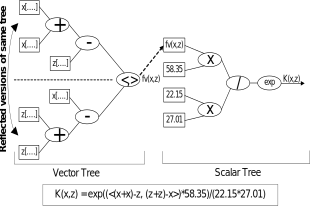
\includegraphics[scale=1.2]{figures/graphs/2-howley}
\label{fig:2-howley}
\caption{Przykładowe drzewo wygenerowane przez algorytm KTree (rysunek pochodzi z pracy \cite{Howley:2002:evolutionary}). Po  lewej stronie widać część wektorową, po prawej część skalarną. Funkcja reprezentowana przez to drzewo to $   e^{\dotp{(x+x)-z}{(z+z)-x}*58.35 / (22.15*27.01)} $}
\end{figure}
Rok później ci sami autorzy zaprezentowali ulepszoną wersję swojego podejścia, tym razem zwaną \emph{KTree} \cite{Howley:2002:evolutionary}. W podejściu tym drzewo reprezentujące generowany kernel składa się z dwóch części: wektorowej i skalarnej. Część wektorowa znajduje się na dole drzewa, zawiera jego liście, będące wektorami cech oraz funkcje operujące na wektorach, takie jak dodawanie i odejmowanie wektorów. Podobnie jak w poprzedniej wersji algorytmu buduje się drzewo symetryczne do wygenerowanego i oblicza ich iloczyn skalarny. Jego wynik, wraz z terminalami zawierającymi losowe stałe, stanowią liście drugiej części drzewa, która zawiera operacje wektorowe. Dzięki zastosowaniu takiej reprezentacji możliwe jest modelowanie za jej pomocą standardowych funkcji jądrowych, takich jak RBF. Przykład takiego drzewa pokazano na rysunku \ref{fig:2-howley}.
W pracy przebadano 3 różne funkcje fitness: dwie oparte na błędzie klasyfikacji zbioru uczącego, jako tiebreak używające kolejno wielkości drzewa oraz sumy współczynników $ \alpha $: $ \sum_{i=1..m}\alpha_i $ oraz trzecią: opartą na 3-krotnej cross walidacji na zbiorze uczącym z wielkością drzewa jako tiebreaker-em. Dodatkowo autorzy testowali użycie "filtra Mercera" (\english{Mercer filter}). Jeśli dla podzbioru danych uczących macierz $ K = (k(x,z)_{i,j=1}^N) $ ma ujemne wartości własne, to filtr przypisuje funkcji jądrowej $ k $ najgorszą możliwość fitness tym samym eliminując funkcje nie spełniające warunków narzuconych przez teorię Mercera.
W przeprowadzonych przez autorów eksperymentach metoda KTree osiągała na większości z 9 przetestowanych zbiorów danych wyniki lepsze lub porównywalne do SVM ze standardowymi kernelami. Najlepszą funkcją fitness okazała się potrójna walidacja krzyżowa. Użycie filtra Mercera okazało się nie wpływać korzystnie na fitness ani osiąganą trafność klasyfikacji, jednak autorzy ostrzegają przed użyciem algorytmu bez filtra Mercera ze względu na groźbę przeuczenia.

\subsubsection{Evolutionary Kernel Machine}
Oryginalne podejście do problemu przedstawia metoda definicja{Evolutionary Kernel Machine }(\akronim{EKM}), przedstawiona w 2006 roku w \cite{gagne_genetic_2006}. Funkcje jądrowe generowane są za pomocą GP, przy czym zbiór terminali stanowią funkcje operujące na wektorach a zwracające wartości skalarne (np. iloczyn skalarny, norma euklidesowa maksimum/minimum z wartości), natomiast wewnętrzne węzły pochodzą ze zbioru funkcji operujących na wartościach skalarnych i zwracających wartości skalarne. Co nietypowe w tym podejściu, to funkcja fitness, która pochodzi z miary oceny marginesu zaproponowanej w \cite{Gilad-Bachrach:2004:MBF:1015330.1015352} a używanej oryginalnie do oceny marginesu w algorytmie 1-NN:
$$ F(K) = \frac{1}{m} \sum_{i=1}^m \delta_K(x_1^{'}, y_i^{'}) - l $$,
gdzie $l$ to wielkość \emph{zbioru prototypów}, a $m$ to wielkość \emph{zbioru walidującego}.

Wyrażenie $ \delta_K(x,y) $ występujące w powyższym wzorze można przedstawić jako $ \delta_K(x,y) = n(x,y) - p(x,y) $. Aby obliczyć $n(x,y)$ oraz $p(x,y)$ należy posortować przykłady ze zbioru prototypów $\{(x_1,y_1),...(x_m, y_m)\}$ względem podobieństwa do przykładu $(x, y)$. $p(x,y)$ oznacza najniższą na posortowanej liście przykładów pozycję przykładu należącego do klasy $y$, czyli tej samej klasy co przykład $(x,y)$, $n(x,y)$ oznacza zaś najniższą pozycję przykłady należącego do klasy innej niż $y$.
Miara podobieństwa, według której sortowane są przykłady pochodzi używa wygenerowanej funkcji jądrowej i wzorowana jest na algorytmie \emph{Kernel-NN} \cite{Yu:2002:KNA:607789.607852}:
$$ d_K(x, x')^2 = K(x, x) + K(x', x') - 2K(x, x') $$
Podsumowując: autorzy aby ocenić funkcje jądrowe na użytek algorytmu SVM, używają ich do skonstruowania klasyfikatora \emph{Kernel-NN} i oceniają margines w tym algorytmie przy pomocy zbioru walidującego.
Dodatkowo, oprócz ewolucji kerneli, autorzy stosują kooperatywną koewolucję zbioru prototypów ze zbiorem kerneli oraz koewolucję typu żywiciel-pasożyt zbioru walidującego ze zbiorem kerneli.
Wyniki eksperymentów zaprezentowane w artykule pokazują porównanie błędów klasyfikacji otrzymanych za pomocą algorytmów $ k-NN $, tradycyjnego \emph{SVM} z jądrem RBF i metody \emph{EKM}. W przypadku 2 z 6 przebadanych zbiorów danych algorytm \emph{EKM} okazał się istotnie statystycznie lepszy od pozostałych dwóch algorytmów.

\subsubsection{Kernel GP}
W 2007 roku ukazał się artykuł autorstwa Seana Luke-a (autora m.in. wykorzystanej w tej pracy biblioteki ECJ \cite{sean_ecj_2010}) i Keith Sullivan opisujący algorytm definicja{Kernel GP }(\akronim{KGP}) \cite{sullivan_evolving_2007}. Algorytm ten, podobnie jak opisane powyżej algorytmy, wykorzystuje programowanie genetyczne do wygenerowania funkcji jądrowych, jednak jako jedyny gwarantuje, że powstałe w ten sposób kernele będą spełniać warunki poprawności definiowane przez teorię Merera. Jest to możliwe dzięki własności zamknięcia zbioru kerneli ze względu na określone operacje. Własność ta umożliwia konstruowanie poprawnych funkcji jądrowych poprzez łączenie funkcji już istniejących (o których wiadomo, że są poprawne) za pomocą określonych operacji. W algorytmie \emph{Kernel GP} zbiór terminali to zbiór trzech standardowych funkcji jądrowych: wielomianowej, sigmoidalnej i gaussowskiej. Zbiór wewnętrznych węzłów drzewa stanowią operacje dodawania, mnożenia przez stałą, mnożenia oraz funkcja wykładnicza. Ponieważ funkcje jądrowe jako argumenty przyjmują wektory a zwracają wartości skalarne, operacje łączące kernele zaś przyjmują i zwracają wartości skalarne, autorzy użyli (opisanego w części \ref{ssec:inicjalizacja}) silnie typowanego programowania genetycznego, żeby zapewnić zgodność typów danych przekazywanych w drzewie.
Jako funkcji fitness autorzy używają wyników 10-krotnej walidacji krzyżowej na zbiorze trenującym.
W eksperymentach autorzy porównali trafność klasyfikacji wydzielonego zbioru testującego przez algorytm \emph{Kernel GP} oraz \emph{Grid Search} (opis w części \ref{ssec:hyperopt}) użyty do SVM z jądrem gaussowskim. Dla połowy z przebadanych wzorów lepsze wyniki osiągnął \emph{Kernel GP}, dla drugiej \emph{Grid Search}.


%\section{Obrazowanie mózgu przy pomocy rezonansu magnetycznego}
%\begin{itemize}
%\item \definicja{Obrazowanie metodą rezonansu magnetycznego} (\akronim{MRI}, \english{Magnetic Resonance Imaging})
%\item \definicja{Obrazowanie metodą funkcjonalnego rezonansu magnetycznego} (\akronim{fMRI}, \english{functional Magnetic Resonance Imaging})
%\end{itemize}
\clearpage